\section{Date: 2026-11-08}
\noindent \textbf{Series ID: APU0400711211} 

\noindent This series is titled Average Price: Bananas (Cost per Pound/453.6 Grams) in the West Census Region - Urban and has a frequency of Monthly. The units are U.S. Dollars and the seasonal adjustment is Not Seasonally Adjusted.The observation start date is 1980-01-01 and the observation end date is 2026-09-01.The popularity of this series is 2. \\ 

\noindent \textbf{Series ID: MESTMACHMANQGSP} 

\noindent This series is titled Chain-Type Quantity Index for Real GDP: Machinery Manufacturing (333) in the Mideast BEA Region and has a frequency of Annual. The units are Index 2017=100 and the seasonal adjustment is Not Seasonally Adjusted.The observation start date is 1997-01-01 and the observation end date is 2025-01-01.The popularity of this series is 1. \\ 

\subsection{Raw Regression}
\noindent Regresses the two series against each other directly. A significant result here can come just as easily from both series sharing a long-run trend as from any real relationship.

\begin{center}
\begin{tabular}{lclc}
\toprule
\textbf{Dep. Variable:}             & value\_fred\_MESTMACHMANQGSP & \textbf{  R-squared:         } &     0.445   \\
\textbf{Model:}                     &             OLS              & \textbf{  Adj. R-squared:    } &     0.425   \\
\textbf{Method:}                    &        Least Squares         & \textbf{  F-statistic:       } &     21.68   \\
\textbf{Date:}                      &       Sun, 08 Nov 2026       & \textbf{  Prob (F-statistic):} &  7.67e-05   \\
\textbf{Time:}                      &           17:18:00           & \textbf{  Log-Likelihood:    } &   -113.18   \\
\textbf{No. Observations:}          &                29            & \textbf{  AIC:               } &     230.4   \\
\textbf{Df Residuals:}              &                27            & \textbf{  BIC:               } &     233.1   \\
\textbf{Df Model:}                  &                 1            & \textbf{                     } &             \\
\textbf{Covariance Type:}           &          nonrobust           & \textbf{                     } &             \\
\bottomrule
\end{tabular}
\begin{tabular}{lcccccc}
                                    & \textbf{coef} & \textbf{std err} & \textbf{t} & \textbf{P$> |$t$|$} & \textbf{[0.025} & \textbf{0.975]}  \\
\midrule
\textbf{const}                      &     200.5465  &       20.614     &     9.729  &         0.000        &      158.250    &      242.843     \\
\textbf{value\_fred\_APU0400711211} &    -155.5450  &       33.406     &    -4.656  &         0.000        &     -224.088    &      -87.002     \\
\bottomrule
\end{tabular}
\begin{tabular}{lclc}
\textbf{Omnibus:}       &  2.716 & \textbf{  Durbin-Watson:     } &    0.630  \\
\textbf{Prob(Omnibus):} &  0.257 & \textbf{  Jarque-Bera (JB):  } &    1.932  \\
\textbf{Skew:}          &  0.632 & \textbf{  Prob(JB):          } &    0.381  \\
\textbf{Kurtosis:}      &  3.011 & \textbf{  Cond. No.          } &     19.9  \\
\bottomrule
\end{tabular}
%\caption{OLS Regression Results}
\end{center}

Notes: \newline
 [1] Standard Errors assume that the covariance matrix of the errors is correctly specified.

\begin{figure}
\centering
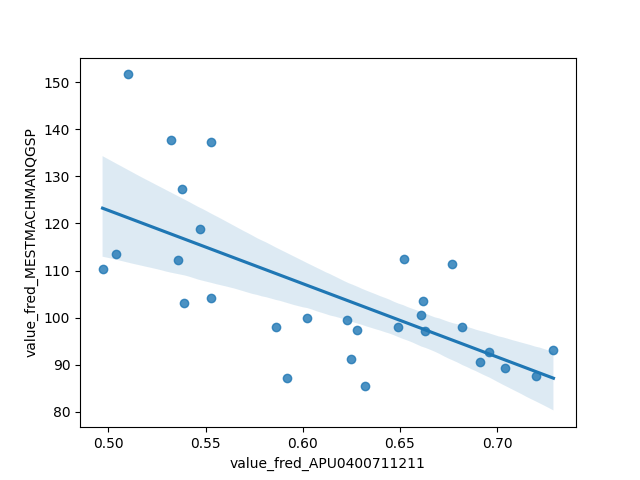
\includegraphics[scale = 0.9]{plots/plot_2026-11-08.png}
\caption{Raw Regression Plot for 2026-11-08}
\end{figure}
\newpage
\subsection{Detrended Regression}
\noindent Regresses the residuals of each series after removing its own linear time trend, so a shared trend can no longer drive the result on its own. A relationship that stays significant here is better evidence of a genuine link between the two series.

\begin{center}
\begin{tabular}{lclc}
\toprule
\textbf{Dep. Variable:}                        & value\_fred\_MESTMACHMANQGSP\_detrended & \textbf{  R-squared:         } &     0.015   \\
\textbf{Model:}                                &                   OLS                   & \textbf{  Adj. R-squared:    } &    -0.021   \\
\textbf{Method:}                               &              Least Squares              & \textbf{  F-statistic:       } &    0.4153   \\
\textbf{Date:}                                 &             Sun, 08 Nov 2026            & \textbf{  Prob (F-statistic):} &    0.525    \\
\textbf{Time:}                                 &                 17:18:00                & \textbf{  Log-Likelihood:    } &   -109.86   \\
\textbf{No. Observations:}                     &                      29                 & \textbf{  AIC:               } &     223.7   \\
\textbf{Df Residuals:}                         &                      27                 & \textbf{  BIC:               } &     226.5   \\
\textbf{Df Model:}                             &                       1                 & \textbf{                     } &             \\
\textbf{Covariance Type:}                      &                nonrobust                & \textbf{                     } &             \\
\bottomrule
\end{tabular}
\begin{tabular}{lcccccc}
                                               & \textbf{coef} & \textbf{std err} & \textbf{t} & \textbf{P$> |$t$|$} & \textbf{[0.025} & \textbf{0.975]}  \\
\midrule
\textbf{const}                                 &    -2.54e-12  &        2.058     & -1.23e-12  &         1.000        &       -4.222    &        4.222     \\
\textbf{value\_fred\_APU0400711211\_detrended} &     -35.1716  &       54.578     &    -0.644  &         0.525        &     -147.156    &       76.813     \\
\bottomrule
\end{tabular}
\begin{tabular}{lclc}
\textbf{Omnibus:}       &  2.209 & \textbf{  Durbin-Watson:     } &    0.735  \\
\textbf{Prob(Omnibus):} &  0.331 & \textbf{  Jarque-Bera (JB):  } &    1.004  \\
\textbf{Skew:}          & -0.114 & \textbf{  Prob(JB):          } &    0.605  \\
\textbf{Kurtosis:}      &  3.883 & \textbf{  Cond. No.          } &     26.5  \\
\bottomrule
\end{tabular}
%\caption{OLS Regression Results}
\end{center}

Notes: \newline
 [1] Standard Errors assume that the covariance matrix of the errors is correctly specified.

\begin{figure}
\centering
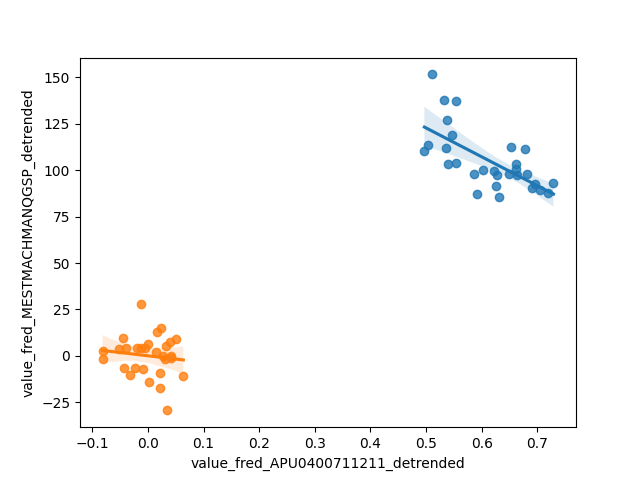
\includegraphics[scale = 0.9]{plots/plot_2026-11-08_detrended.png}
\caption{Detrended Regression Plot for 2026-11-08}
\end{figure}
\newpage
